% Methodology section

\subsection{Opetopes}

Originally developed in higher category theory \citep{cheng2004higher, kock2010polynomial}, opetopes are higher-dimensional shapes defined recursively by their boundaries, which are themselves opetopes of lower dimensions. Dimensions here refer to the number of vertices in the opetope, with a 0-dimensional opetope being a point, a 1-dimensional opetope being a directed edge, and so on. Opetopes of higher dimensions are constructed from lower-dimensional opetopes by gluing them together along their boundaries. To further simply using an example, an opetope can be a 2D square going along clockwise, thus not only capturing the shape but also the directionality of the shape.

\begin{figure}[htbp]
    \centering
    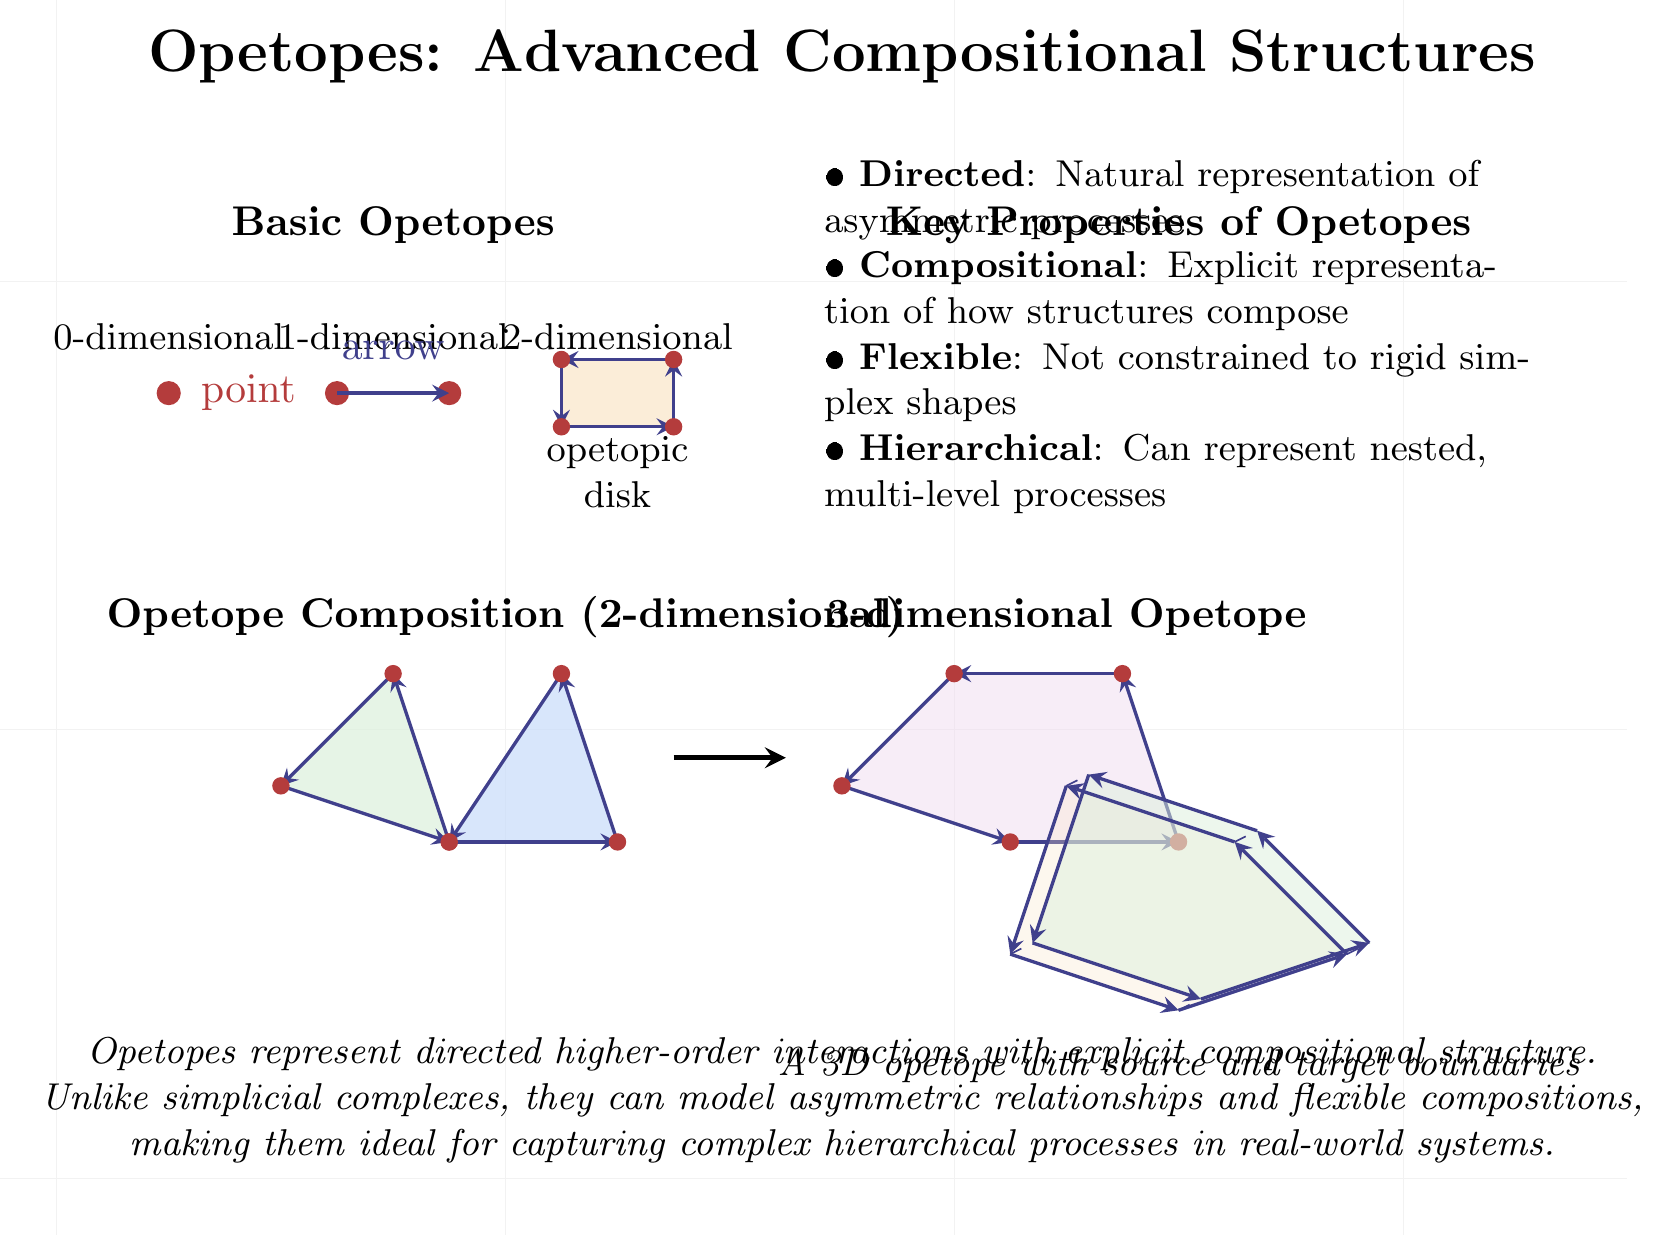
\includegraphics[width=\textwidth]{figures/opetope_structures-1.png}
    \caption{Visual representation of opetopes and their properties. Top: Basic opetopes of different dimensions from 0D to 2D, along with key properties that distinguish them from simplicial complexes.}
    \label{fig:opetope_structures}
\end{figure}

\subsubsection{Formal Definition}

Formally, an $n$-dimensional opetope can be defined as:

\begin{itemize}
    \item A 0-dimensional opetope is a point
    \item A 1-dimensional opetope is a directed arrow between points
    \item For $n>1$, an $n$-dimensional opetope has:
    \begin{itemize}
        \item A source boundary, consisting of $(n-1)$-dimensional opetopes arranged in a tree-like pattern
        \item A target boundary, consisting of a single $(n-1)$-dimensional opetope
    \end{itemize}
\end{itemize}

The mathematical framework of opetopes is closely related to operads, higher categories, and polynomial functors \citep{baez2020network, leinster2004higher}. These connections provide rich analytical tools for understanding opetopic models.

Opetopes can be formalized in dependent type theory \citep{finster2019opetopic}, providing a foundation for mechanical verification of opetopic models. This connection bridges opetopic modeling with formal logic and programming language theory. In this work, we use Lean the theorem prover to model opetopes and show how to use them to construct complex systems models.
